%In order to create the map, we use the SLAM developed by our colleges in Rescue team at the Georg-Simon-Ohm University of applied science. The SLAM itself is based on the iterative closest point (ICP) algorithm and laser data provided by the front-mounted Hokuyo URG04-LX laser scanner. Then we base the localization on the amcl package provided by ROS.

The arena at RoboCup$@$work is virtually unchanged during the competition. Therefore, a SLAM approach is unnecessary. Since industrial production sites have in general a static layout, this assumption is justified. However, a SLAM algorithm is required to generate the initial map, or update the information to add smaller changes.

The Autonohm RoboCup Rescue team deploys successfully a self developed SLAM approach, ohm\_tsd\_slam. The referring ROS package is based on a 3D/2D reconstruction and localization framework which has been subject of May~et.~al.~\cite{May2014}. Additional work by Koch~et.~al.~\cite{Koch2015}, aimed at multi-source-SLAM and loop closing capabilities. 

In order to build maps of the RoboCup$@$work arena, only data of a 2D LIDAR is required. In an iteration, the SLAM framework first reconstructs an artificial laser scan out of the map from the last known robot pose, using a raycasting implementation. 

In the second step, a scan matching algorithm based on the Iterative Closest Points (ICP) algorithm (Chen and Medioni \cite{chen:icp}, Besl et. al. \cite{bsl:icp}, Zhang \cite{zhang:icp} and Random Sample Consensus (RANSAC) algorithm (Fischler et. al. \cite{Fischler:ransac})) estimates the transformation between the reconstructed laser data and and the current scan. This pose change is applied to the last known pose and results in the new localization of the robot. 

The map is being updated from the new acquired robot pose and converted in a ROS compatible data format (occupancy grid) in the last step. This step is necessary as the ohm\_tsd\_slam package uses an abstract representation based on Signed Distance Functions (SDF) (Curless et. al. \cite{curless:sdf}), which is incompatible to standard ROS packages. Figure~\ref{fig:slam_map_expl} depicts a map generated by ohm\_tsd\_slam.

\begin{figure}[h!]
\begin{center}
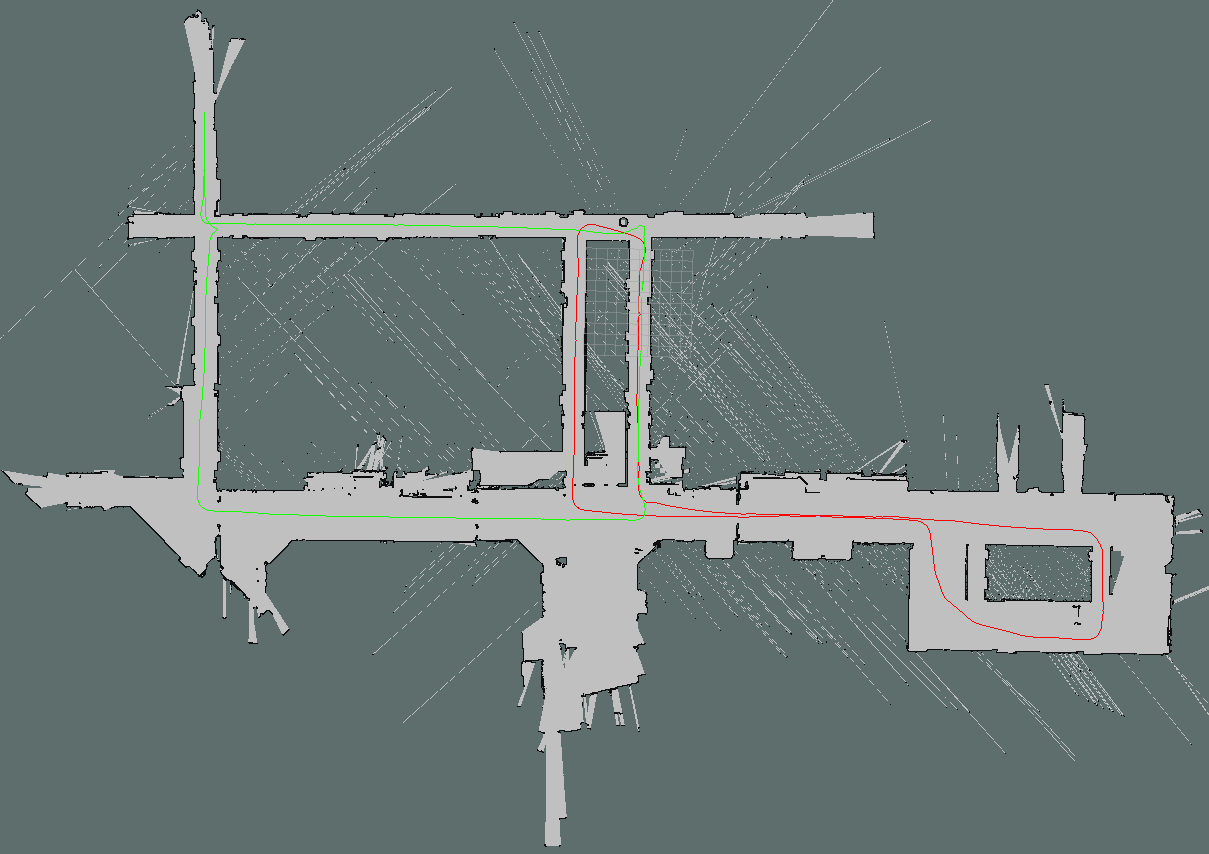
\includegraphics[width=0.9\textwidth]{img/multislam_big.png}
\end{center}
\caption{Mapping Example. Image depicts the resulting map of two cooperating robots. The red and green lines illustrate the estimated trajectory of both units. This map shows an additional feature of ohm-tsd-slam, the approach is able to map comparably large areas as the reconstructed map had an edge length of \unit[122]{m}. \textit{Source: Koch et. al.\cite{Koch2015}.}}
\label{fig:slam_map_expl}
\end{figure}


More information and a git repository regarding the 2D single or multi-SLAM ROS package ohm\_tsd\_slam can be found on the referring ROS Wiki page \cite{ohmtsdslam:ros}.

%what should come here:
%\todo{Phils part...}
%\begin{enumerate}
%	\item describe our slam algo
%	\item describe improvements from last robocup
%	\item picture from a map
%	\item refs to our tsd papers \cite{May2014}, \cite{Koch2015}
%	\item github source
%\end{enumerate}
